\documentclass{article} 

\usepackage{ctex}

\usepackage{graphicx}

\usepackage{geometry}
%rfr 可以参考geometry的官方手册:https://ftp.kddilabs.jp/CTAN/macros/latex/contrib/geometry/geometry.pdf

%* 以下命令也可以放置到geometry宏包的可选参数中
%! 以下命令一定要放在导言位置
\geometry{
    showframe,
        %* 在默认情况下,即页面区域只包含文本区域,不包含页眉、页脚、侧页边,这一参数的效果是显示文本区域的边线、整个页眉部分、页脚的上边线以及侧页边的左边线;如果设置页面区域包含其他部分,则同时会显示相应地部分
        %! 注意,在设置这一参数时,页眉/页脚和侧页边根据是否被包括进页面区域的不同条件,会有各自不同的显示效果:(1)不管页眉和页脚是否被包括进页面区域,设置该参数都会显示整个页眉部分和页脚部分;(2)即使侧页边没有被包括在页面区域内,设置该参数依然会显示侧页边的左边线,一旦侧页边被包括进页面区域内,则还会显示其右边线,这一点和页脚不同
    showcrop,
        %* 显示裁剪标志
%% paper
%% 这一部分也可以在"\documentclass[options]{style}"命令的可选参数中设置(包括twoside和twocolumn)
    paper = a4paper,  
        % 也可以设置名称为"papername"
        %* 设置提前定义好的纸张尺寸,可以选择的值包括:[a0--a6、b0--b6、c0--c6]paper、b0j--b6j、ansi[a--e]paper、letterpaper、executivepaper、legalpaper、screen等
        %rfr 关于纸张尺寸,这里简要说明一下国际标准化组织(International Organization for Standardization,简称ISO)定义的A、B、C系列纸张的尺寸:在同一字母序列内,从0开始到6,数字越大,纸张越小;相同的字母序列内,A系列纸张最小,B系列纸张最大,C系列纸张介于两者之间,可以参考维基百科的介绍:https://zh.wikipedia.org/wiki/ISO_216
    % papersize={20cm,20cm}, 
        %* 自定义尺寸,设置格式是{<width>,<height>},如果只设置一个值,则代表宽度和高度都设置为这一个值(下面涉及同时设置宽度和高度时,同样遵循这个规则),也可以单独设置paperwidth或者paperheight
        %! 经检验,如果同时设置了paper和papersize,以papersize参数为准
    % landscape,  
        % 也可以加上布尔逻辑值:landscape = true,其效果等于portrait = false(下面涉及类似的参数时,同样遵循这个规则)
        %* 设置横向纸张,默认值为"portrait",即纵向纸张
%% layout
%% "layout"的效果实际是在原来的纸张区域和页面区域之间多加一层矩形区域,在默认情况下,该区域的左上角紧贴原来纸张区域的左上角,在大多数情况下,并不需要设置这一参数
    % layout = a5paper,
        %* 根据上面提到的"layout"的定义,这一区域的尺寸一般小于原来纸张的尺寸
    % layoutsize = {20cm,20cm},
        %* 同时设置该区域的宽度和高度,也可以单独设置layoutwidth或者layoutheight
        %! 同样地,如果同时设置layout和layoutsize,以layoutsize参数为准
    % layoutoffset = {5cm,5cm},
        %* 设置该区域的左边线和原来纸张的左边线之间的距离以及该区域的上边线和原来纸张的上边线之间的距离,也可以单独设置layouthoffset或者layoutvoffset
%% (total)body
%% geometry将这一部分的参数称为"body size",但随后又说明其实包含了整个"total body"(页面)的相关参数
    % scale=.5, 
        % 效果等同于(total)width = .5\paperwidth、(total)height = {{0.5,0.5}\paperheight
        %* 同时设置页面宽度和纸张宽度的比值以及页面高度和纸张高度的比值,两者默认值都为0.7,也可以单独设置hscale或者vscale
    % total = {15cm,15cm},
        %* 同时设置页面宽度和页面高度,也可以单独设置totalwidth或者totalheight
        %! 注意,和paperwidth、paperheight、textwidth、textheight这些参数不同,这些参数都有对应的"\paperwidth"、"\paperheight"、"\textwidth"、"\textheight"命令,代表当前的纸张宽度、纸张高度、文本宽度、文本高度,(total)width和(total)height参数并不存在对应的"\(total)width"和"\(total)height"命令,因此在代码中如果使用这两个并不存在的命令,会导致汇编报错(但是在设置箱子的相关参数时,却可以使用"\width"、"\height"等命令,但此时这两个命令分别指的是箱子自适应时的宽度和高度,和此处的页面宽高度没有关系)
    % text = {10cm,10cm},
        % 也可以设置名称为"body"
        %* 同时设置文本宽度和文本高度,也可以单独设置textwidth或者textheight
    % lines = 5,
        %* 通过设置每页的行数来设置文本高度
    includeall,
        %* 是否包含页眉(head)、页脚(foot)、侧页边(marginalpar,来自"marginal paragraph"的缩写),其他可以选择的值有"includefoot"、"includeheadfoot"、"includemp"、"includeall",以及将各个值中的"include"改为"ignore"之后的值
        %! 吴康隆P60称“默认的选项为includehead,表示总文本区包含页眉”,这句话其实是有问题的,geometry宏包的官方手册在"includehead"参数后面明确提到,这一项默认设置为false,因此默认情况下其实页眉、页脚和侧页边都没有被包含在页面内
        %! 注意,这一参数只是控制页眉、页脚、侧页边是否被包括进页面区域,也就是未来的【现实打印区域】,而页眉、页脚和侧页边的内容样式则由fancyhdr宏包提供的"\pagestyle{}"命令进行设置(如plain、headings等),如果没有设置内容样式,则不管是否设置了此处的"includeall"参数,也不会在LaTeX的打印效果中显示页眉、页脚和侧页边的内容(当然,某些文档类,比如ctexart提前定义了页眉样式,因此即使不使用"\pagestyle{}"命令进行设置,也会现实页眉)
%% totalbody&margin
%% 下面这一参数可以同时设置页面和页边距,但是geometry将"total body"误作了"body"
    % divide = {3cm,15cm,}
        %* 同时设置水平方向上的页面左边距、页面宽度、页面右边距,以及竖直方向上的页面上边距、页面高度、页面下边距,一般只需要设置其中两项,另外剩下的一项系统会通过纸张宽度/高度和这两项的差值自动计算出来,也可以单独设置hdivide或者vdivide
%% margin
    % left = 3cm,
        % 也可以设置名称为"lmargin",在双边模式下也可以设置名称为"inner"
        %* 设置页面左边距
        %? geometry宏包提到这个参数不同于原生命令中的"leftmargin",但暂时还不知道"leftmargin"代表的是哪一段距离
        %* 相应地,也可以设置页面右边距:"right/rmargin/outer"
    % top = 3cm,
        % 也可以设置名称为"tmargin"
        %* 设置页面上边距
        %? geometry宏包提到这个参数不同于原生命令中的"topmargin",但暂时还不知道"topmargin"代表的是哪一段距离
        %* 相应地,也可以设置页面下边距:"bottom/bmargin"
    % margin = {3cm,2cm},
        %* 同时设置水平方向上的页面左边距和页面右边距,以及竖直方向上的页面上边距和页面下边距,也可以但单独设置hmargin或者vmargin
    % marginratio = 3:2,
        % 也可以设置名称为"ratio",设置的值应该表现为小于100的正整数比,并且用":"符号连接
        %* 同时设置水平方向上的页面左边距和页面右边距的比值,以及竖直方向上的页面上边距和页面下边距的比值,前者的默认值在单边模式下为1:1,在双边模式下为2:3,后者的默认值为2:3,也可以单独设置hmarginratio或者vmarginratio
    % centering,
        %* 效果相当于marginratio = 1:1,也可以单独设置hcentering(在单边模式下这是默认值)或者vcentering,要注意此处的"centering"并不是在浮动体环境中经常使用的"\centering"命令
    % twoside,
        % 这一部分也可以在"\documentclass[options]{style}"命令的可选参数中设置
        %* 设置"twoside"(双边)参数会区分"inner"(近书脊)和"outer"(远书脊)两个参数,这两个参数也可以仍然沿用默认情况下的"left"和"right",但是后面这对概念在双边模式下容易导致误解:在奇数页,"inner/left"代表了左页边,"outer/right"代表了右页边;而在偶数页,"inner/left"代表了右页边,"outer/right"代表了左页边,因此在双边模式下不如使用不容易引起误解的"inner"和"outer"参数,具体到打印效果,则侧页边的位置在奇数页会显示在页面左侧,在偶数页会显示在页面右侧,由于book/report文档类默认双边模式,因此这一参数通常用于article文档类
    % asymmetric,
        % 这一部分也可以在"\documentclass[options]{style}"命令的可选参数中设置
        %* 和"twoside"参数的效果相反,这一参数使侧页边始终出现在页面右侧,由于article文档类默认单边模式,因此这一参数通常用于book/report文档类
    % bindingoffset = 1cm,
        %* 在单边模式下,从纸张的左边线分出相应宽度的矩形范围作为装订区域,页面左边距相应减少;在双边模式下,从纸张的内侧边线分出相应宽度的矩形范围作为装订区域,页面内侧边距相应减少。geometry宏包在前后两处关于分出的宽度是否属于页面左边距/页面内侧边距存在矛盾,但实际效果是相同的,这里取其中一种说法
%% native dimentions
%% 下面这部分内容存在于LaTeX的原生命令中,geometry宏包也包括了这些参数
    % head = 2cm,
        % 也可以设置名称为"headheight"
        %* 设置页眉高度
    % headsep = 1cm,
        %* 设置页眉边距
    % foot = 2cm,
        % 也可以设置名称为"footskip"
        %* 设置页脚边距
    % marginparwidth = 4cm,
        %* 设置侧页边宽度
    % marginparsep = 1cm,
        %* 设置侧页边边距
    % nohead,
        %* 移除页眉,效果等同于head = 0pt, headsep = 0pt,如果页眉没有被包括进页面区域,该参数只会导致页眉被移除,如果页眉被包括进页面区域,该参数会导致页面上边线延伸至原来页眉的上边线处
    % nofoot,
        %* 移除页脚,效果等同于foot = 0pt,如果页脚没有被包括进页面区域,该参数只会导致页脚被移除,如果页脚被包括进页面区域,该参数会导致页面下边线延伸至原来页脚的下边线处
    % noheadfoot,
        %* 同时移除页眉和页脚
    % nomarginpar,
        %* 移除侧页边,效果等同于marginparwidth = 0pt, marginparsep = 0pt,如果侧页边没有被包括进页面区域,该参数只会导致侧页边被移除,如果侧页边被包括进页面区域,在单边模式下,该参数会导致页面右边线延伸至原来侧页边的右边线处;在双边模式下,该参数会导致页面外侧边线延伸至原来侧页边的外侧边线处
    % footnotesep = .5cm,
        %* 设置脚注边距
    % twocolumn,
        %* 设置双栏,默认值为"onecolumn",即单栏
    % columnsep = 1cm,
        %* 双栏模式下,设置左栏右边线和右栏左边线之间的距离
    % offset = {3cm,4cm},
        %* 同时设置页面左边距和页面上边距,也可以单独设置hoffset或者voffset
    % reversemp,
        % 也可以设置名称为"reversemarginpar"
        %* 在单边模式下,使边注始终显示在页面左侧;在双边模式下,使边注显示的位置与原来相反:在奇数页上显示在左侧,在偶数页上显示在右侧,也即从原来的显示在页面外侧改为显示在页面内侧
        %! 注意,如果设置了showframe参数,会发现此时设置reversemp参数会导致页面发生了移动,但是侧页边的位置并没有移动到相反的位置,尽管如此,可以通过在正文中设置边注来检验边注显示的位置发生了翻转
    }

\usepackage[colorlinks,linkcolor=blue]{hyperref}

\begin{document}
如果要深刻理解geometry宏包,应该首先熟悉该宏包的官方手册\footnote{\url{https://ftp.kddilabs.jp/CTAN/macros/latex/contrib/geometry/geometry.pdf}}定义的一些排版术语,下面提供geometry宏包中提供的排版示意图(\ref{geometry_documentation_figure})。以下涉及到的重要排版术语首次出现时,均标为粗体,并且在后面的括号中提供临时拟定的翻译。

\begin{figure}
    \centering
    \fbox{
        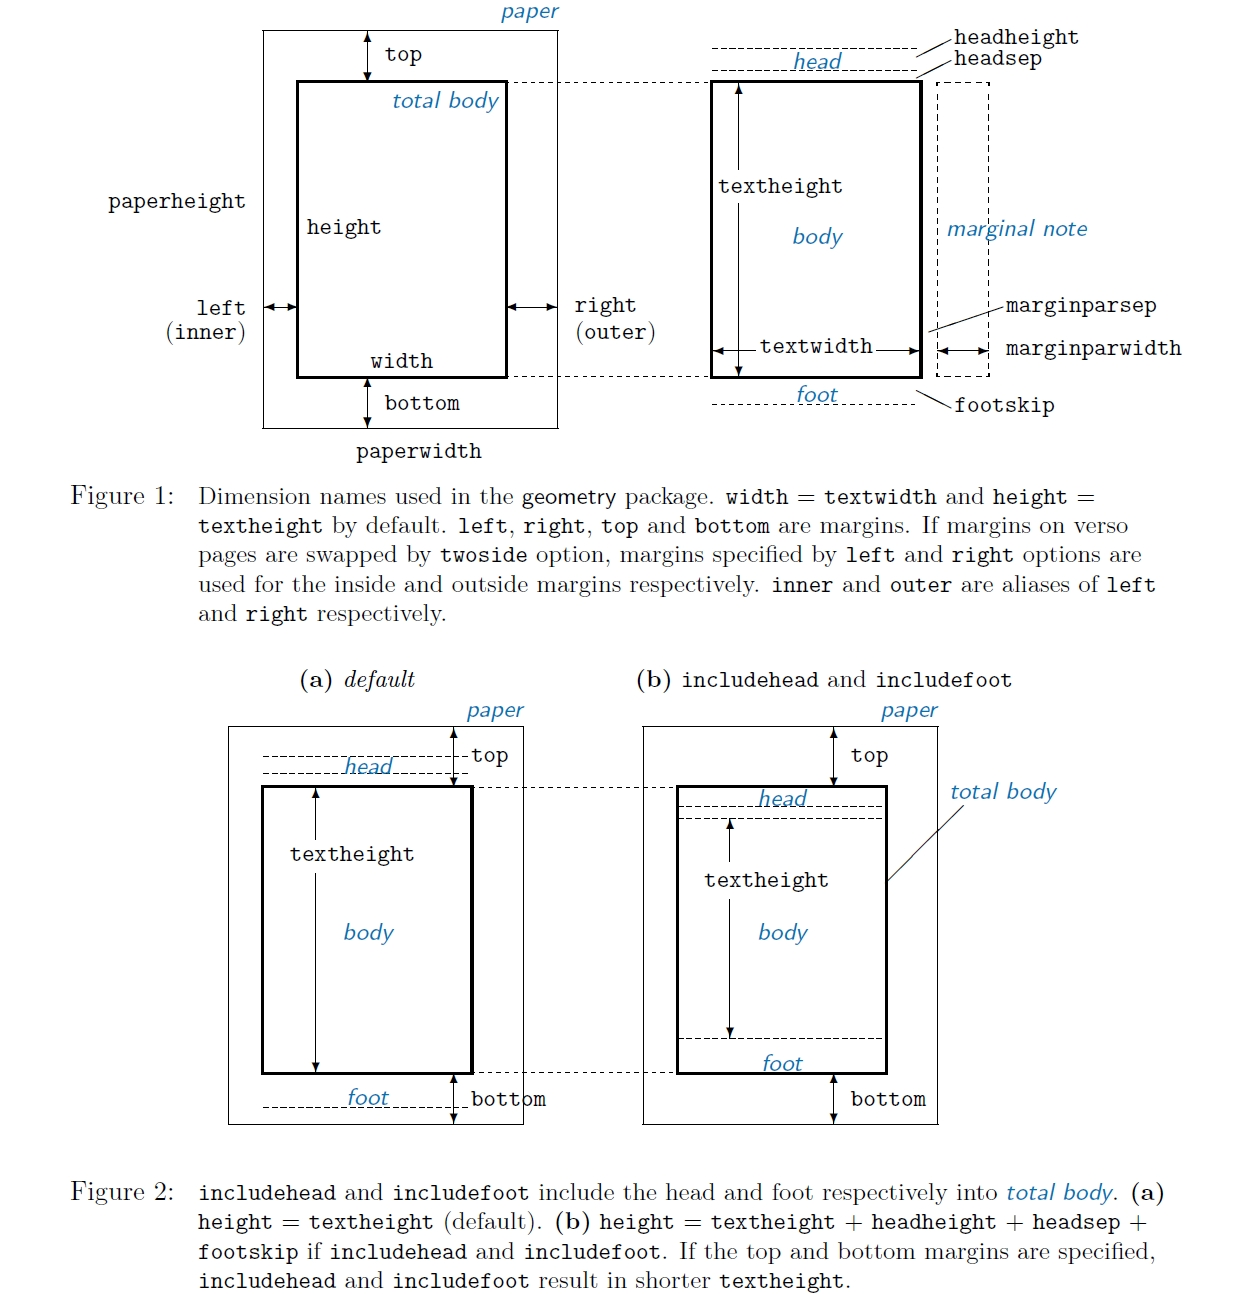
\includegraphics[width = .8\textwidth]{geometry_figure.png}
    }
    \caption{Geometry宏包中提供的排版示意图}
    \label{geometry_documentation_figure}
\end{figure}

geometry宏包的官方手册中提供的示意图并没有包括\textbf{``crop mark''(裁剪标志)}以及相关的一些概念(尽管手册在下文提及了宏包包含设置crop mark的命令),下面提供几张谷歌上的相关示意图(\ref{google_crop_mark})。
%* 此处的"crop"并不是名词“作物”的意思,而是动词“裁剪”的意思

\begin{figure}
    \centering
    \fbox{
        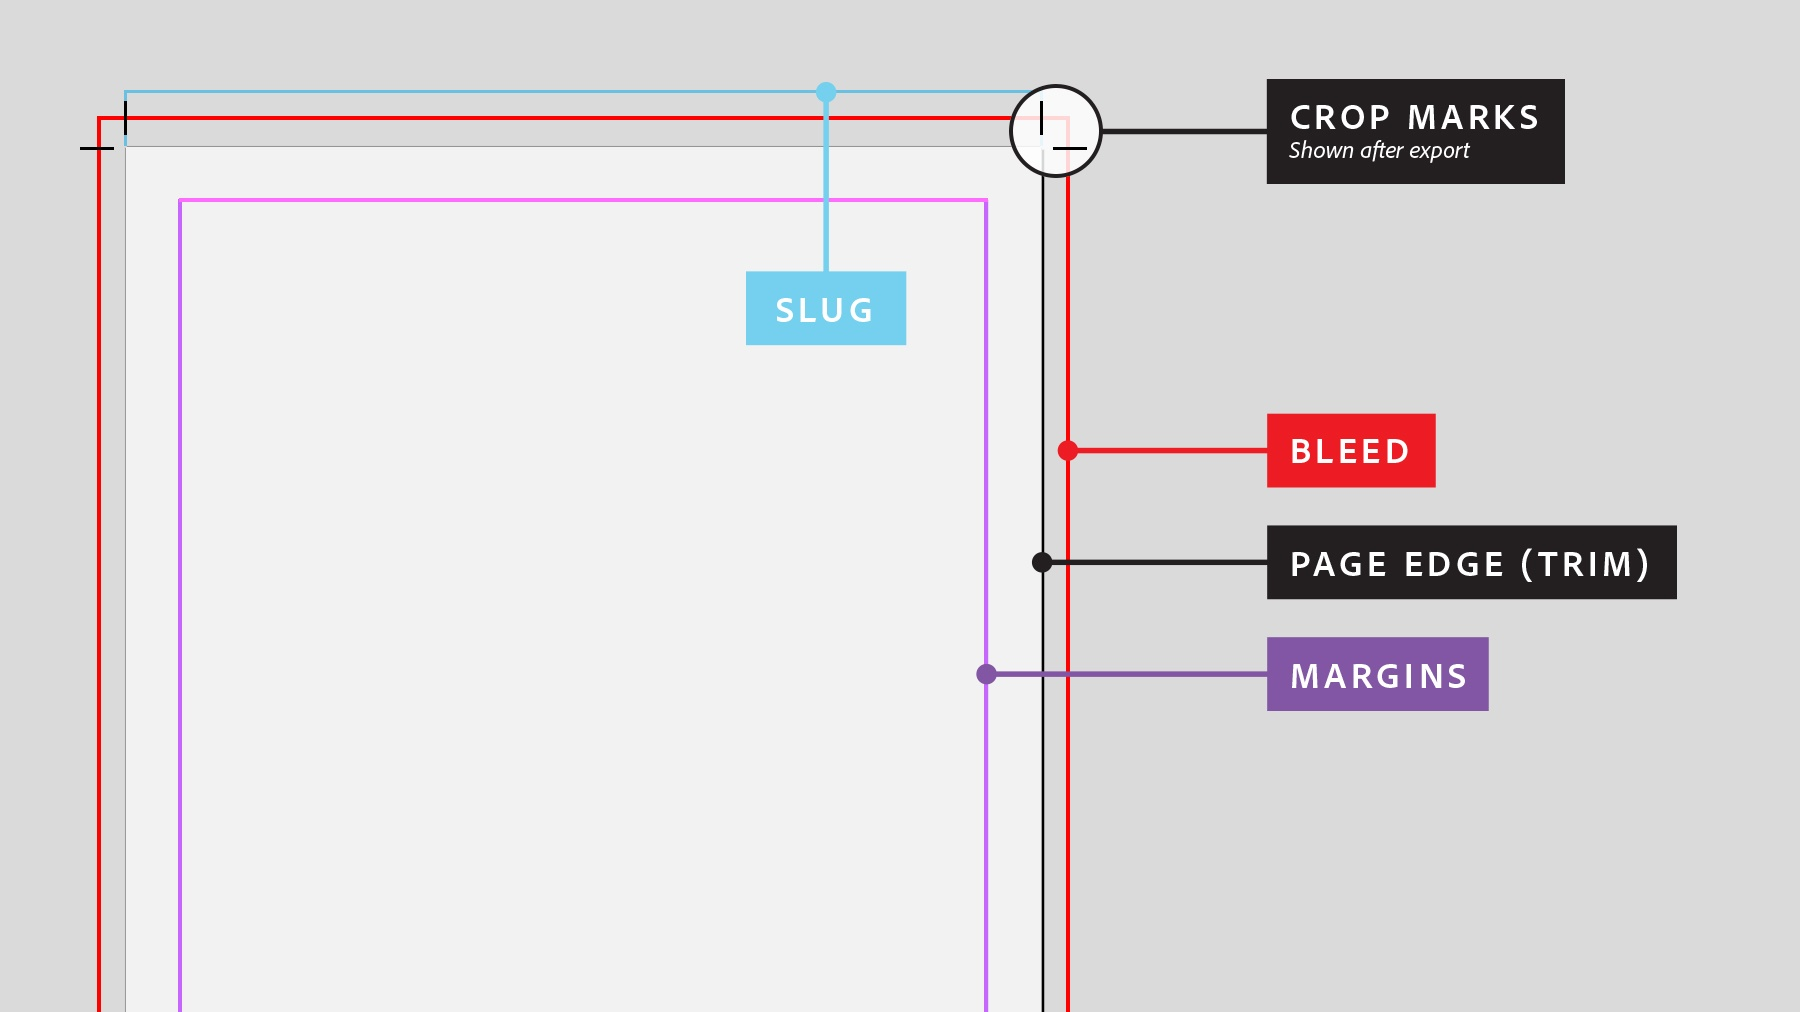
\includegraphics[width = .8\textwidth]{crop_marks_1.jpg}
    }
    \\
    \fbox{
        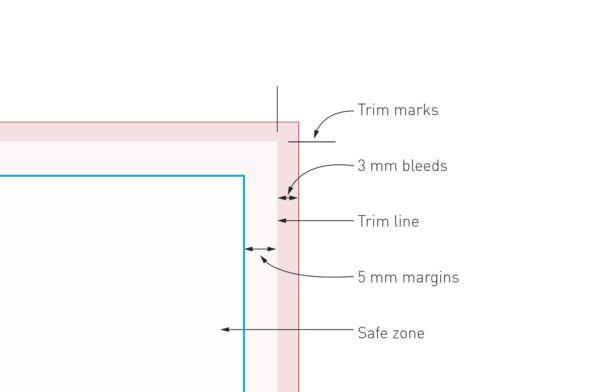
\includegraphics[width = .8\textwidth]{trim_marks_2.jpg}
    }
    \\
    \fbox{
        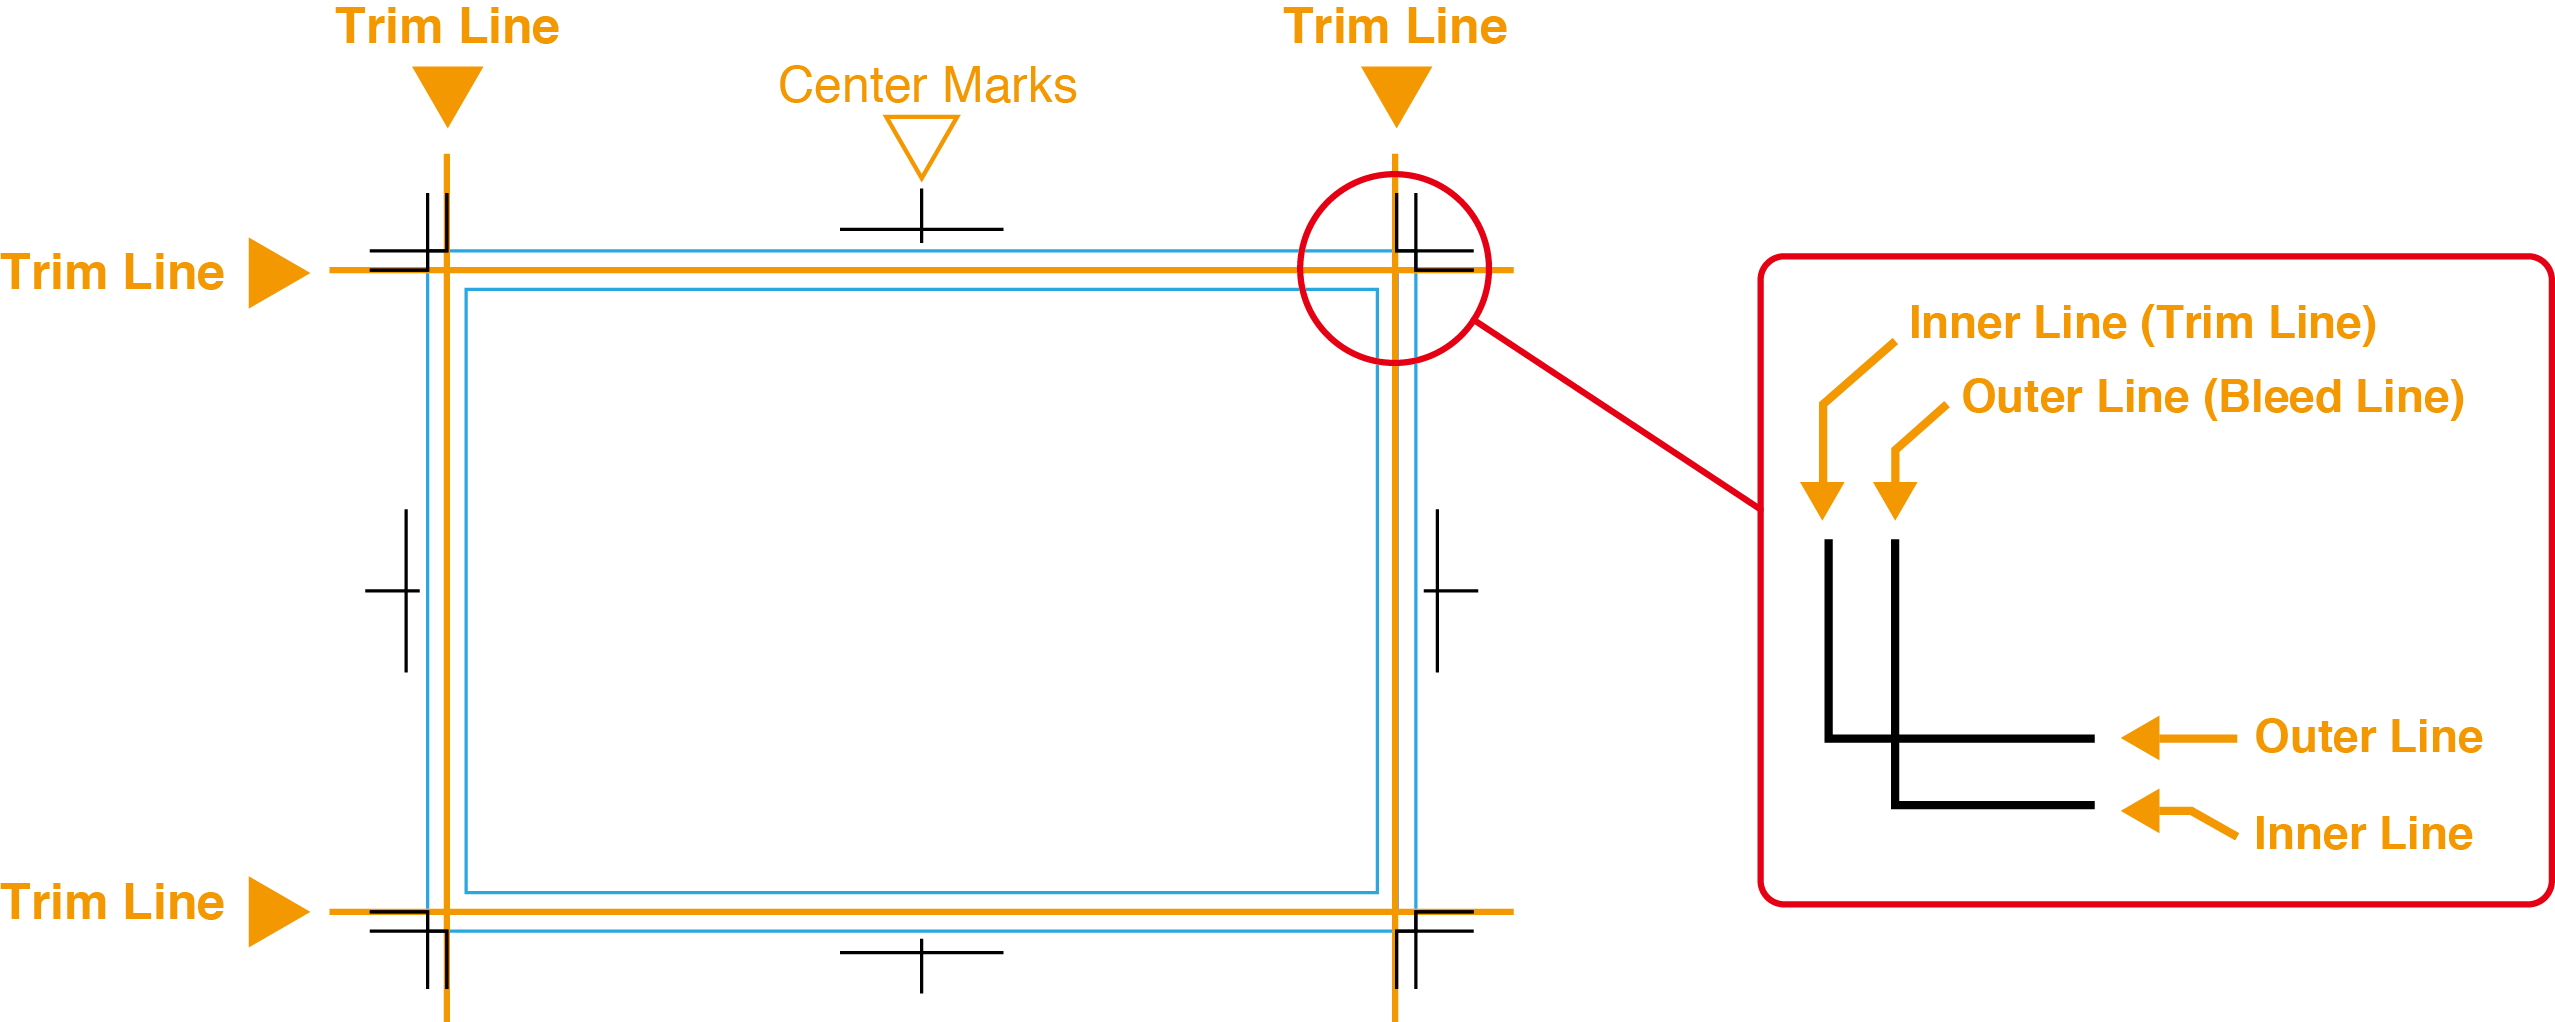
\includegraphics[width = .8\textwidth]{trim_marks_1.png}
    }
    \caption{谷歌上有关``crop mark''概念的相关示意图}
    \label{google_crop_mark}
\end{figure}

可以发现,``crop mark''也可以称为``trim mark'',一般位于\textbf{``paper''(纸张)}区域内的四个角落处,或者表现为两条不相交的垂直短线,或者呈直角状\footnote{有时候,在纸张的四条边内侧的中间还会各有四条线段,线段中间可能会有一条垂直的短线,或者有一个穿过线段的圆圈。},框出一个小于纸张大小的矩形区域,称为\textbf{``total body''(页面)},在打印出来的纸张有裁剪的需要时,这个页面区域就是裁剪后剩下的部分,裁剪掉的部分称为\textbf{``bleed''(废血)},页面的边线称为``trim line''(页面边线),也可以称为``page edge''。有的时候,在纸张区域的四个角落处会出现两个相同的标记,此时位于内侧的两根短线构成``inner crop mark'',位于外侧的两根短线构成``outer crop mark'',但其实只有``inner crop mark''才是真正的裁剪标记,其框出的范围才是页面区域,而``outer crop mark''框出的范围则介于页面区域和纸张区域之间,其边线称为``bleed line''\footnote{这个``bleed line''和上文的``bleed''并没有什么关系,``bleed line''位于``bleed''区域的内部。},这个区域有些类似于geometry宏包提供的可供设置的"layout"区域,似乎并没有什么实际的作用。
%rfr 关于inner crop mark和outer crop mark,网上的相关介绍也不多,可以参考这个网站上的简短说明:https://support.ricoh.com/bb_v1oi/pub_e/oi_view/0001044/0001044134/view/users/int/0088.htm
% rfr 关于bleed line、trim line和caution line(下文会提到)这几个概念,可以参考下面这个网站上的小视频:https://www.printplace.com/blog/graphic-design-friday-trim-and-bleed-lines/?srsltid=AfmBOopRlj9aoBbFiPC5JGmbdY1NQkLvhsW4Y2-bkA_jenIikXBnvAc8

这样,我们就暂时得到了两个矩形区域:纸张区域(paper)和页面区域(total body),他们通过裁剪标记(crop mark)分隔开来。纸张的四边和页面的四边之间各自形成了四段距离统称为\textbf{``margin''(页面边距)},分别称为\textbf{``top''(页面上边距)}、\textbf{``bottom''(页面下边距)}、\textbf{``left''(页面左边距)}和\textbf{``right''(页面右边距)},在\textbf{``twoside''(双边)}模式\footnote{这是book、report文档类的默认模式,article文档类需要通过可选参数设置。}下,页面的左右边距会根据奇偶页的不同而来回交替:在奇数页的页面左边距就是偶数页的页面右边距,奇数页的页面右边距就是偶数页的页面左边距,为了避免混淆,geometry宏包将前两对距离统一称为\textbf{``inner''(页面内侧边距)},将后两对距离统一称为\textbf{``outer''(页面外侧边距)}\footnote{但是在双边模式下,也可以继续使用``left''和``right''的称呼,但是此时其表示的不再是字面意义上的左和右,而是分别等同于``inner''和``outer'',即内和外,这是由第一页,也是所有的奇数页上的格局决定的。}。纸张和页面还各自有宽度参数和高度参数,纸张的宽度称为\textbf{``paperwidth''(纸张宽度)},纸张的高度称为\textbf{``paperheight''(纸张高度)},页面的宽度称为\textbf{``(total)width''(页面宽度)},页面的高度称为\textbf{``(totalheight)''(页面高度)}。因此可以得到下面两个关系:
\begin{itemize}
    \item paperwidth = (total)with + left/inner + right/outer
    \item paperheight = (total)height + top + bottom
\end{itemize}

现在再将范围缩小到页面。在页面内部,可能存在的部分有:\textbf{``body''(文本)}\footnote{这也就是放置\LaTeX 的document环境当中除去页眉、页脚和边注以外的其他所有内容的区域,由于这部分包含了文本最重要的主体部分,一般不允许这部分内容超出该区域,因此该区域有时候也被称为``safe zone''(安全区)。}、\textbf{``header''(页眉)}、\textbf{``footer''(页脚)}、\textbf{``marginal note''(侧页边)},之所以说是``可能'',是因为在geometry宏包的默认设置中,页面只包含了文本区域,可以通过设置``inclue/ignore + 其他页面部分''参数来包括或者排除相关的部分。其中,页眉的高度称为\textbf{``head(height)''(页眉高度)},页眉下边线和文本上边线之间有一段距离,称为\textbf{``headsep''(页眉边距)};文本区域的下边线到页脚基线的高度称为\textbf{``foot(skip)''(页脚边距)}\footnote{页脚不像页眉那样存在上边线和下边线的分别,因此只需要定义文本区域的下边线和一段垂直距离,就足以确定页脚基线的位置。},顺带一提,geometry宏包还重定义了脚注到正文的间距,称为\textbf{``footnotesep''(脚注边距)}\footnote{在\LaTeX 原生命令中,这一段距离通过``\textbackslash skip\textbackslash footins''命令控制。另外,注意不要混淆``脚注''和``页脚''这两个概念,前者属于文本区域,后者则不属于文本区域。};页边的宽度称为\textbf{``marginpar(width)''(侧页边宽度)},页面左边线(twoside模式下是内侧边线)和文本右边线(twoside模式下是外侧边线)之间的距离称为\textbf{``marginparsep''(侧页边边距)}。文本区域的边线称为``caution line''(文本边线),文本区域也有宽度参数和高度参数,文本的宽度称为\textbf{``textwidth''(文本宽度)},文本的高度称为\textbf{``textheight''(文本高度)}。在默认情况下,即页面只包括文本区域,我们就可以得到下面两个关系:
\begin{itemize}
    \item (total)width = textwidth
    \item (total)height = textheight
\end{itemize}
如果页面同时包含了页眉和页脚,上述高度关系就需要变成:
\begin{itemize}
    \item (total)height = textheight + head(height) + headsep + foot(skip) + footnotesep
\end{itemize}
如果页面包含了侧页边,上述宽度关系就需要变成:
\begin{itemize}
    \item (total)width = textwidth + marginpar(width) + marginparsep
\end{itemize}

\clearpage
1\marginpar[left]{right}

\end{document}